\documentclass[pdftex,11pt]{article}
\usepackage[pdftex]{graphicx}
\usepackage{enumerate}
\usepackage{amsmath}
\usepackage{amssymb}
\usepackage{multicol}
\usepackage{algpseudocode}
\usepackage{algorithm}
\usepackage{hyperref}
\usepackage{algorithm}
\usepackage{algorithm}
\usepackage{geometry}
\usepackage{float}
\geometry{verbose,tmargin=1in,bmargin=1in,lmargin=1in,rmargin=1in}
\begin{document}
\title{COMP 540 - Homework 2}
\author{Xiang Zhou (xz58) and Guangyuan Yu (gy12)}
\title{COMP 540 Statistical Machine Learning HW2}
\maketitle
\newcommand{\pr}{\mathbb{P}}
\section{Gradient and Hessian of $NLL(\theta)$ for logistic regression}
	
	\subsection{}
	\begin{itemize}
	\item
	Given $g(z) = \frac{1}{1 + e^{-z}}$
	\begin{align*}
		\frac{\partial g(z)}{\partial z} &=-1\cdot\frac{1}{(1 + e^{-z})^{2}}\cdot-(e^{-z})\\
						&=\frac{1}{1+e^{-z}}\cdot\frac{1+e^{-z}-1}{1+e^{-z}}\\
						&=g(z)\cdot(1 - g(z))\\
	\end{align*}	
	\end{itemize}
	
	
	\subsection{}
	\begin{itemize}
	\item
	We know $NLL(\theta) = -\frac{1}{m}\sum_{i = 1}^{m} \left( y^{(i)}\text{log}\,h_{\theta}(x^{(i)}) + (1 - y^{(i)})\text{log}\,(1 - h_{\theta}(x^{(i)})) \right)$, 
	\\$\frac{\partial} {\partial \theta} NLL(\theta)= \frac{\partial NLL(\theta)}{\partial h_{\theta}(x^{(i)})} \frac{\partial h_{\theta}(x^{(i)})}{\partial \theta} $, \\
	$h_{\theta}(x^{(i)}) = g(\theta^Tx)$\\
	and given $\frac{\partial g(z)}{\partial z} =g(z)\cdot(1 - g(z))$ from above, we have:\\
	\begin{align*}
		\frac{\partial} {\partial \theta} NLL(\theta) 
		&= -\frac{1}{m}\sum_{i = 1}^{m} \left( \frac{y^{(i)}}{h_{\theta}(x^{(i)})} - \frac{(1 - y^{(i)})}{1 - h_{\theta}(x^{(i)})}\right) x^{(i)} h_{\theta}(x^{(i)})(1 - h_{\theta}(x^{(i)})) \\
			&= -\frac{1}{m}\sum_{i = 1}^{m} (y^{(i)}(1 - h_{\theta}(x^{(i)})) - (1 - y^{(i)})h_{\theta}(x^{(i)}))x^{(i)} \\
			&= \frac{1}{m}\sum_{i = 1}^{m} (h_{\theta}(x^{(i)}) - y^{(i)}) x^{(i)}\\
	\end{align*}
	\end{itemize}

\subsection{}
	\begin{itemize}
	\item To prove that $H$ is positive definite, we want to prove that for any nonzero vector $\textbf{a}$, $\textbf{a}^TH\textbf{a} > 0$. 
	\begin{align*}
	\textbf{a}^TH\textbf{a} &=  \textbf{a}^T X^T S X \textbf{a}\\
		&= \sum_{i = 1}^{d}\sum_{j = 1}^{d} \sum_{k = 1}^{m} a_i x_{ki}(h_{\theta}(x^{(i)}))(1 - h_{\theta}(x^{(i)})) x_{kj} a_j \\
		&= \sum_{i = 1}^{d}\sum_{j = 1}^{d} \sum_{k = 1}^{m} a_i x_{ki}x_{kj} a_j (h_{\theta}(x^{(i)}))(1 - h_{\theta}(x^{(i)})) \\
	\end{align*}	
		
	since $i = j, a_i = a_j , x_{ki} = x_{kj}$\\
	\begin{align*}
		\textbf{a}^TH\textbf{a} &= \sum_{i = 1}^{d} \sum_{k = 1}^{m} a_i^2 x_{ki}^2(h_{\theta}(x^{(i)}))(1 - h_{\theta}(x^{(i)}))            
	\end{align*}
	Given $ (a_i x_{ki} )^2 > 0, (h_{\theta}(x^{(i)}))(1 - h_{\theta}(x^{(i)}) > 0$, we can prove $\textbf{a}^TH\textbf{a} > 0$.\\
	Thus, we have proved that H is positive definite.
	\end{itemize}

\section{Regularizing logistic regression}
\subsection{}
\begin{itemize}
\item \begin{align*}
		\theta_{MLE} &= \text{arg}\max_{\theta}\prod_{i=1}^{m}P(y^{(i)}| x^{(i)}; \theta) \\
		&=  \text{arg}\max_{\theta}\prod_{i=1}^{m}g(\theta^T x^{(i)}) \\
	\end{align*}
	Therefore, we have:
	\begin{align*} 
		\prod_{i=1}^{m}{g(\theta_{MLE}^T x^{(i)})} \geq \prod_{i=1}^{m}{g(\theta^T x^{(i)})}\\
		\prod_{i=1}^{m}\frac {g(\theta_{MLE}^T x^{(i)})}{g(\theta^T x^{(i)})} \geq 1\\
		\prod_{i=1}^{m}\frac {g(\theta_{MLE}^T x^{(i)})}{g(\theta_{MAP}^T x^{(i)})} \geq 1\\
	\end{align*}
	Similarly, we have:
	\begin{align*} 
		\prod_{i=1}^{m}{P(\theta_{MAP})g(\theta_{MAP}^T x^{(i)})} \geq \prod_{i=1}^{m}{P(\theta)g(\theta^T x^{(i)})}\\
		\frac {P(\theta_{MAP})}{P(\theta)} \geq \prod_{i=1}^{m}\frac {g(\theta^T x^{(i)})}{g(\theta^T x^{(i)})}\\
		\frac {P(\theta_{MAP})}{P(\theta_{MLE})} \geq \prod_{i=1}^{m}\frac {g(\theta_{MLE}^T x^{(i)})}{g(\theta_{MAP}^T x^{(i)})} \geq 1 \\
	\end{align*}
	Thus, $P(\theta_{MAP}) \geq P(\theta_{MLE})$. Since, $P(\theta)$ is $N(0, \alpha^2I)$,
	\begin{align*} 
		\frac {1}{\sqrt{2\pi}^{-k}\sqrt{|\alpha^2 I|} } exp ( - \frac{\theta_{MAP}^T\theta_{MAP}}{2\alpha^2}) \geq \frac{1}{\sqrt{2\pi}^{-k}\sqrt{|\alpha^2 I|} } exp ( - \frac{\theta_{MLE}^T\theta_{MLE}}{2\alpha^2}) \\
	\end{align*}
	\begin{align*} 
		- \theta_{MAP}^T\theta_{MAP}  \geq \theta_{MLE}^T\theta_{MLE}\\
		\Vert\theta_{MAP}\Vert_2 \leq \Vert\theta_{MLE}\Vert_2 \\
	\end{align*}
	The proof is done.
\end{itemize}






\section{Inplementing a k-nearest-neighbot classifier}

When $k=1$, we get an $accuracy=137/500=0.274000$.
When $k=5$, we get an $accuracy=142/500=0.284000$.
When we compare one-loop with two-loop, the matrix difference is zero.
When we compare no-loop with two-loop, the matrix difference is zero.
bright rows: It means this test data has low similarity with the majority of the training data. bright columns : It means this training data has low similarity with the majority of the test data.
\subsection{Speeding up distance computations}
Two loop version took 37.736882 seconds.
One loop version took 55.912858 seconds.
No loop version took 0.340704 seconds.

\subsection{Choosing k by cross-validation}
\begin{figure}[H]
  \caption{Choosing k by crossvalidation on the CIFAR-10 dataset}
  \centering
    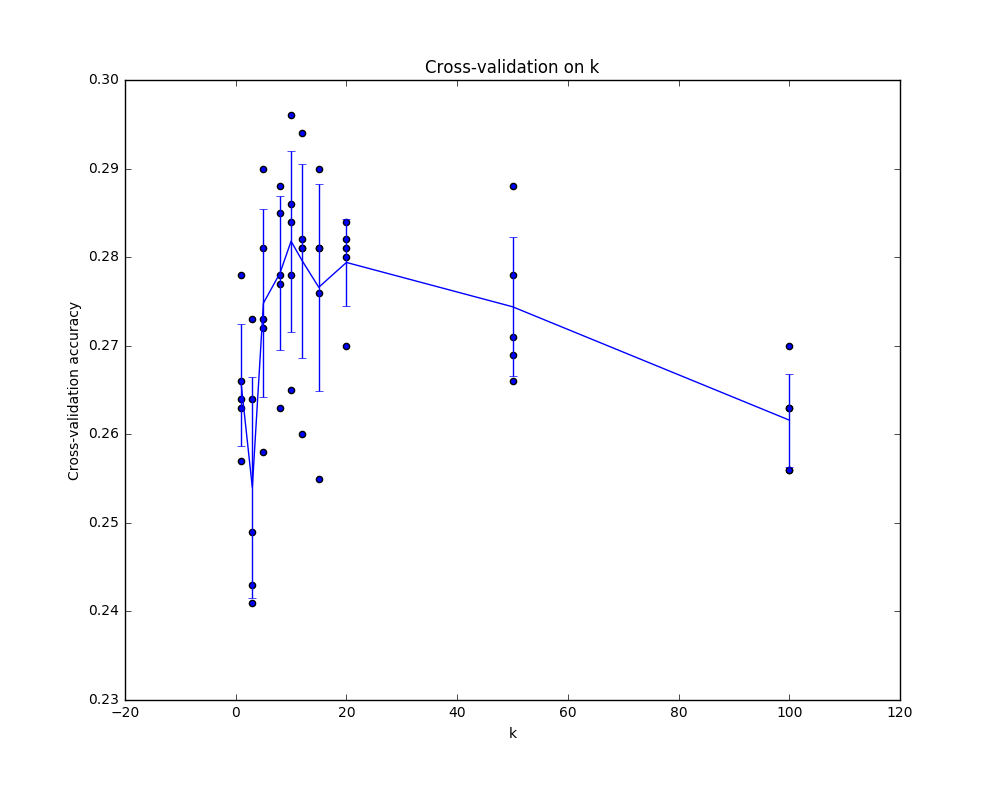
\includegraphics[scale=0.5]{fig1.png}
\end{figure}
We think the best k is $k=3$ and we get $accuracy=139 / 500=0.278000$

\section{Implementing logistic regression}
\subsection{Visualizing the dataset}

\begin{figure}[H]
  \caption{The training data}
  \centering
    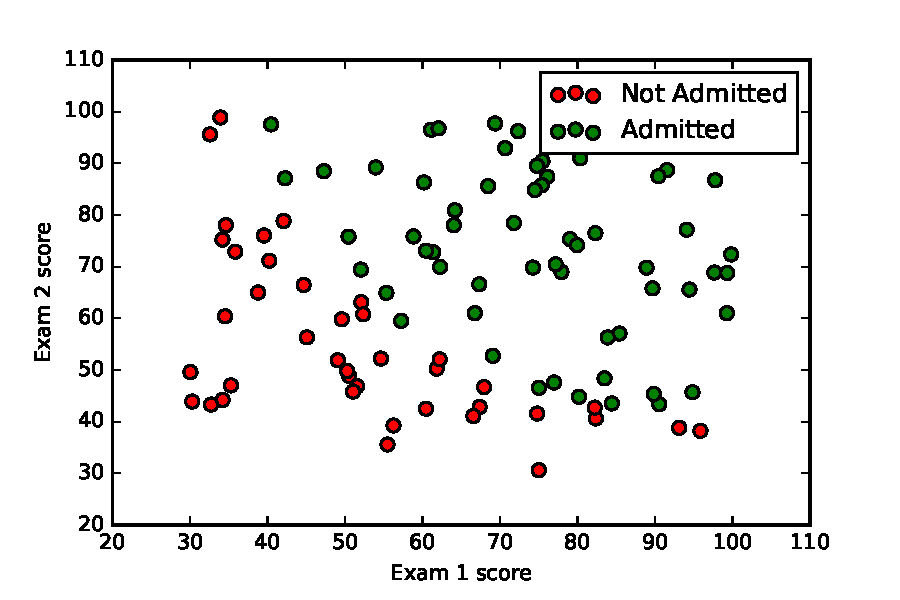
\includegraphics[scale=0.5]{fig1.pdf}
\end{figure}

\subsection{3A1. Implementing logistic regression the sigmoid funciton}
Yes we had tested sigmoid function, it is correct.
\subsection{3A2 Cost function and gradient of logistic regression}
Loss on all-zeros theta vector (should be around 0.693) =  0.69314718056\\
Gradient of loss wrt all-zeros theta vector (should be around [-0.1, -12.01, -11.26]) =  [ -0.1        -12.00921659 -11.26284221]\\
Optimization terminated successfully.\\
         Current function value: 0.203498\\
         Iterations: 19\\
         Function evaluations: 20\\
         Gradient evaluations: 20\\
Theta found by fmin\_bfgs:  $[-25.16056945   0.20622963   0.20146073]$\\
Final loss =  0.203497702351\\

\subsection{Learning parameters using fmin\_bfgs}
\begin{figure}[H]
  \caption{The decision boundary}
  \centering
    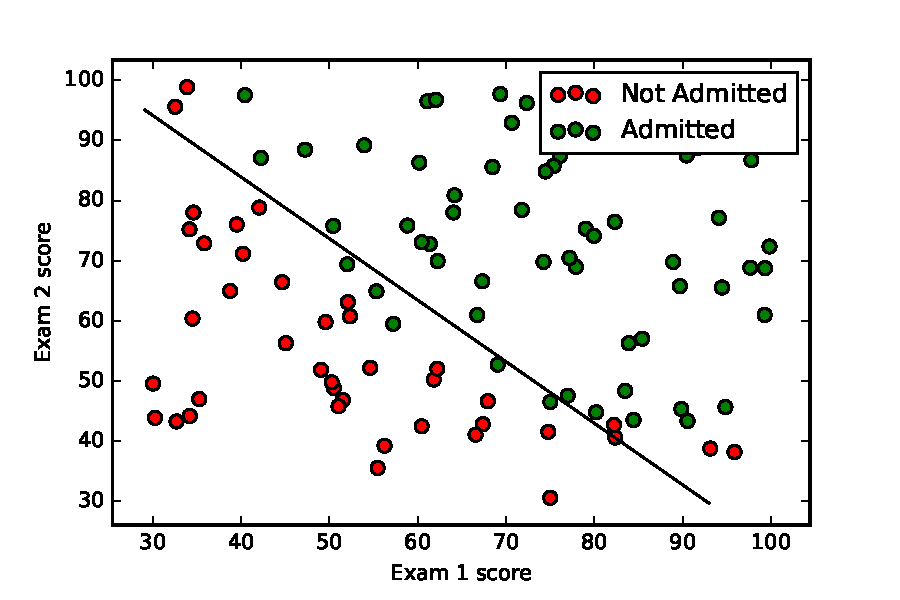
\includegraphics[scale=0.5]{fig2.pdf}
\end{figure}
\begin{figure}[H]
  \caption{The decision boundary from sklearn}
  \centering
    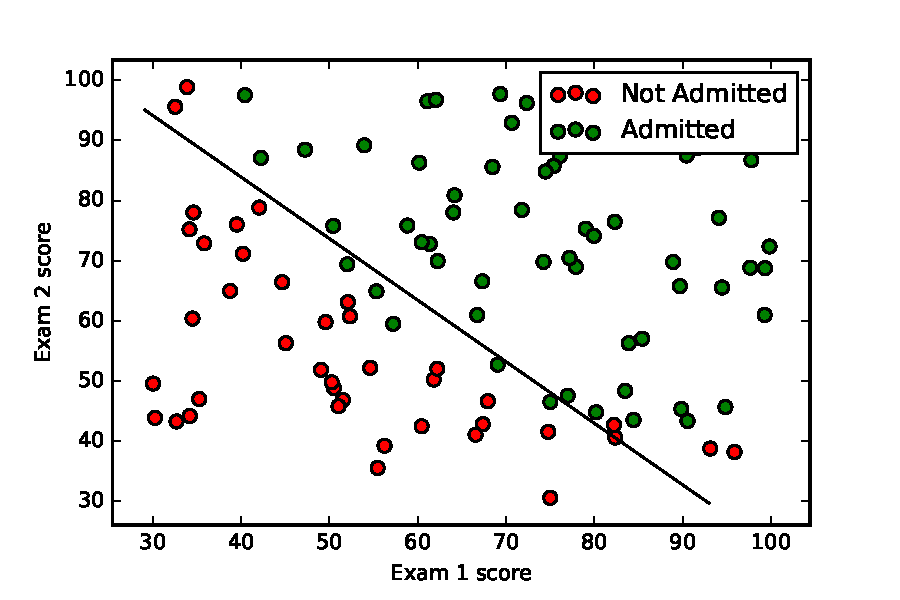
\includegraphics[scale=0.5]{fig2sk.pdf}
\end{figure}
Theta found by sklearn:  [[-25.15293066   0.20616459   0.20140349]]
\subsection{3A3 Prediction using a logistic regression model}
The student with 45/85 score will be admitted with a probability of 0.776246678481.\\
The accuracy on the training set is 0.89.\\

\section{3part B Regularized logistic regression}
\subsection{visualizing the data}

\begin{figure}[H]
  \caption{Plot of training data}
  \centering
    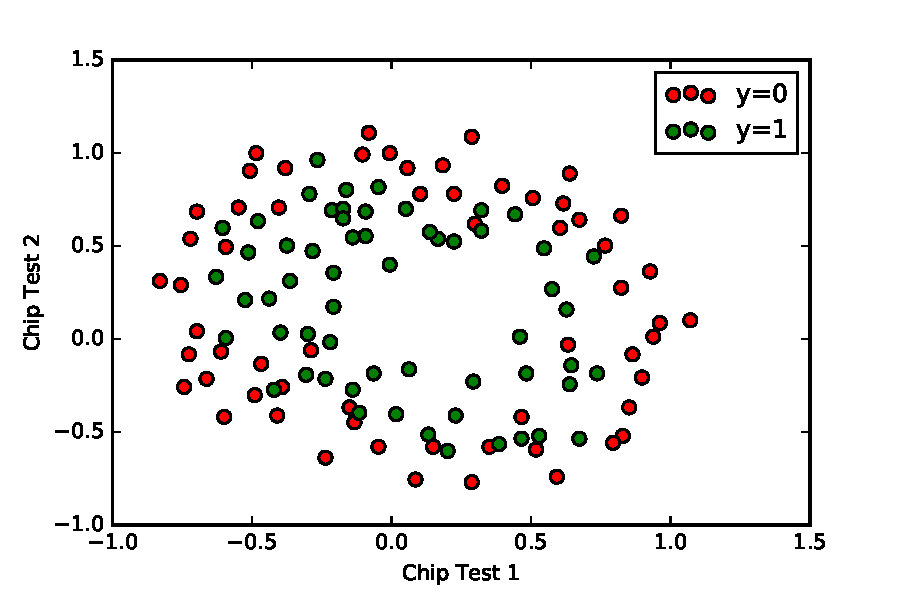
\includegraphics[scale=0.5]{fig3.pdf}
\end{figure}
\subsection{3B1 Cost function and gradient for regularized logistic }

Accuracy on the training set =  0.830508474576
\begin{figure}[H]
  \caption{Traning data with decision boundary for lambda=1}
  \centering
    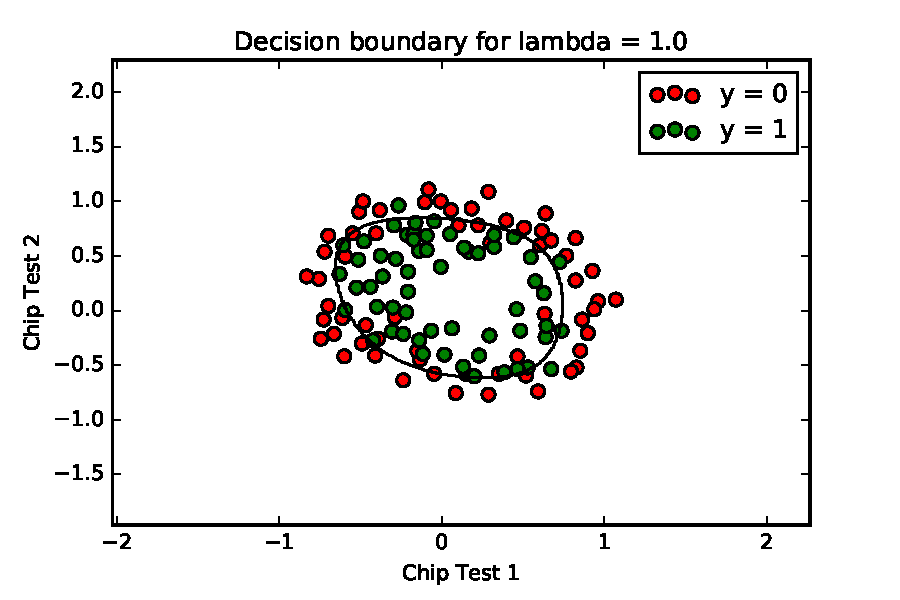
\includegraphics[scale=0.5]{fig4.pdf}
\end{figure}


\subsection{3B2 prediction using the model}

Accuracy on the training set =  0.830508474576





\subsection{3B3 varing lambda}
\begin{figure}[H]
  \caption{lambda=0.1}
  \centering
    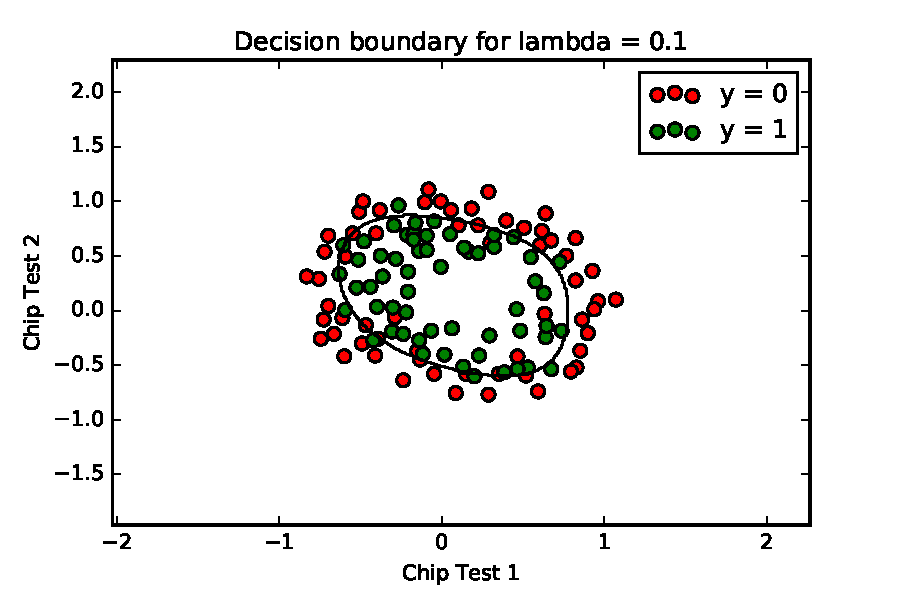
\includegraphics[scale=0.5]{fig401.pdf}
\end{figure}
\begin{figure}[H]
  \caption{lambda=100}
  \centering
    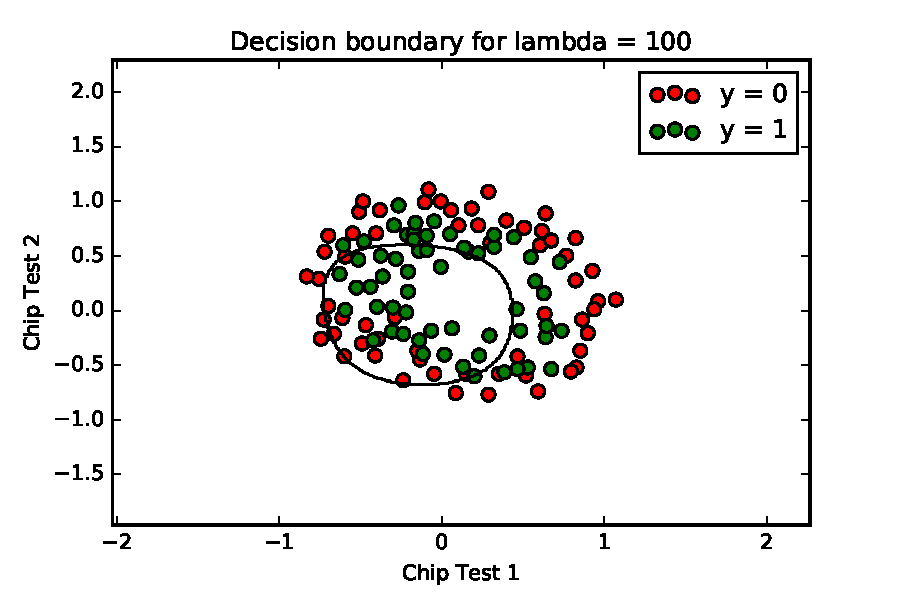
\includegraphics[scale=0.5]{fig4100.pdf}
\end{figure}

\subsection{3B4 Exploring L1 and L2 penalized logistic regression}
\begin{figure}[H]
  \caption{L1sklearn with reg=1}
  \centering
    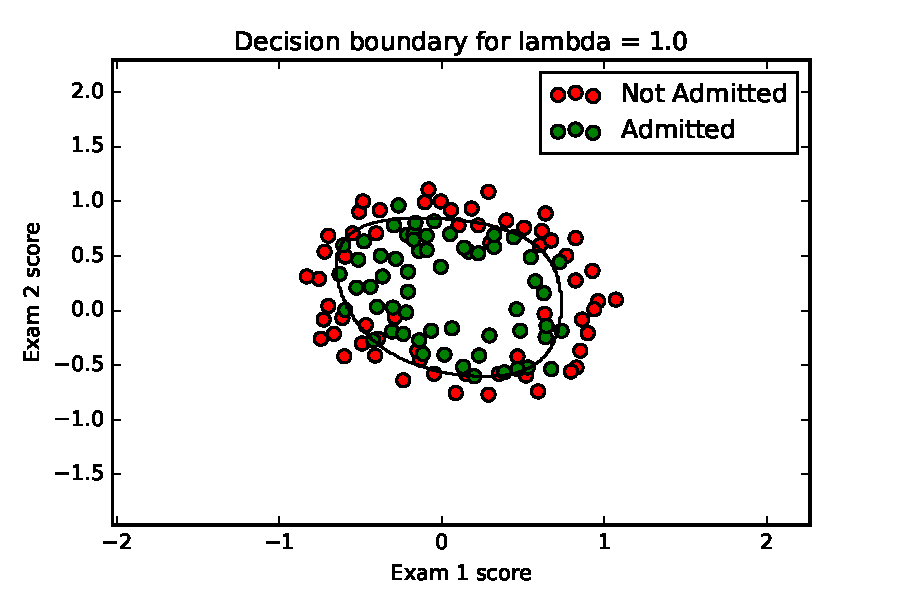
\includegraphics[scale=0.5]{fig4sk.pdf}
\end{figure}
\begin{figure}[H]
  \caption{L1sklearn with reg=0.1}
  \centering
    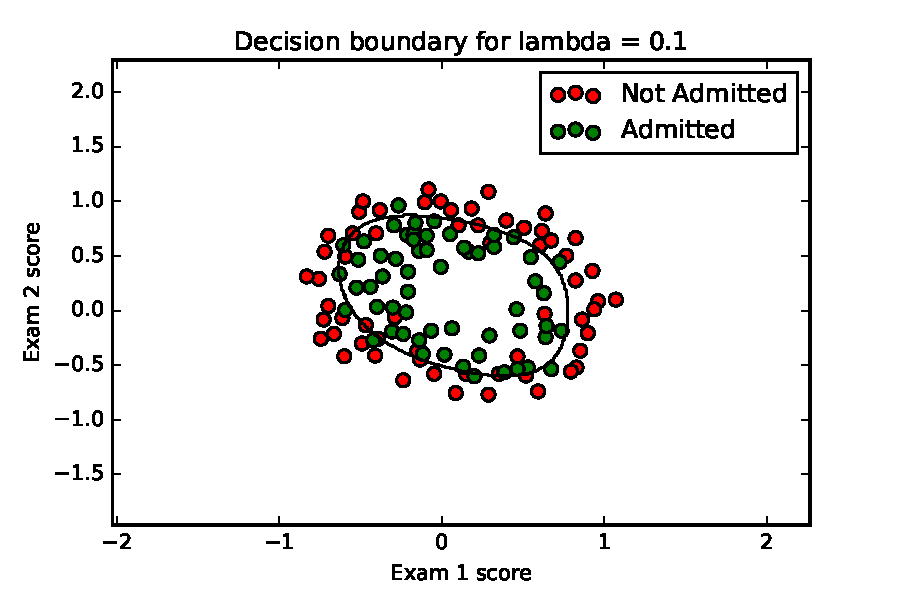
\includegraphics[scale=0.5]{fig4sk01.pdf}
\end{figure}
\begin{figure}[H]
  \caption{L1sklearn with reg=100}
  \centering
    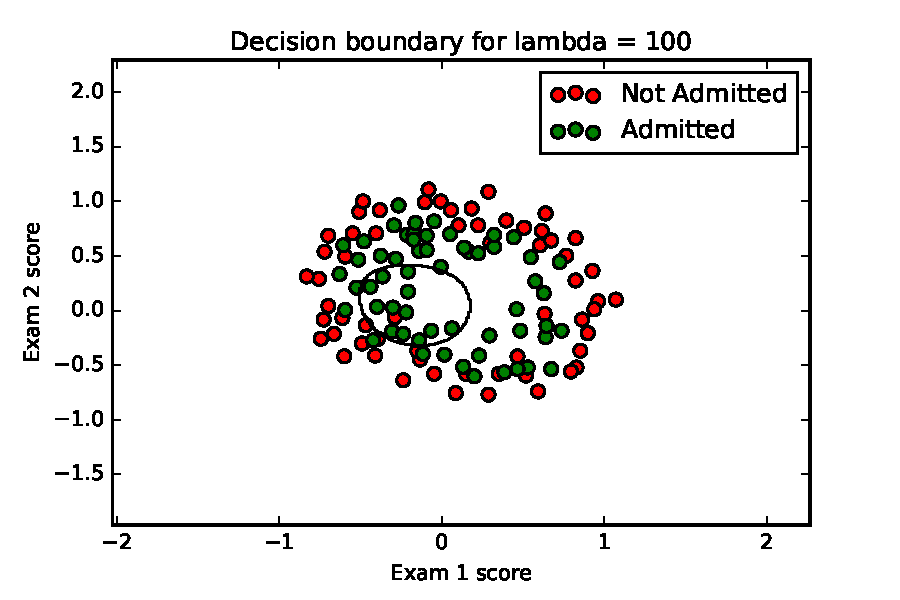
\includegraphics[scale=0.5]{fig4sk100.pdf}
\end{figure}

\subsubsection{with reg=100}
L2sklearn\\
Theta found by sklearn with L2 reg:  [ 0.00468635 -0.01726848  0.0064196  -0.05402665 -0.01327551 -0.03727145
 -0.01821195 -0.00761037 -0.00885306 -0.02224573 -0.04288369 -0.00238585
 -0.01393196 -0.00354828 -0.04072376 -0.02078577 -0.00467203 -0.00354978
 -0.00624894 -0.00500393 -0.03153159 -0.03381515 -0.00108319 -0.00694192
 -0.0003945  -0.00788595 -0.00157683 -0.04058858]
Loss with sklearn theta:  0.68061702032\\
L1\\
Theta found by sklearn with L1 reg:  [ 0.  0.  0.  0.  0.  0.  0.  0.  0.  0.  0.  0.  0.  0.  0.  0.  0.  0.
  0.  0.  0.  0.  0.  0.  0.  0.  0.  0.]\\
Loss with sklearn theta:  0.69314718056
\begin{figure}[H]
  \caption{path}
  \centering
    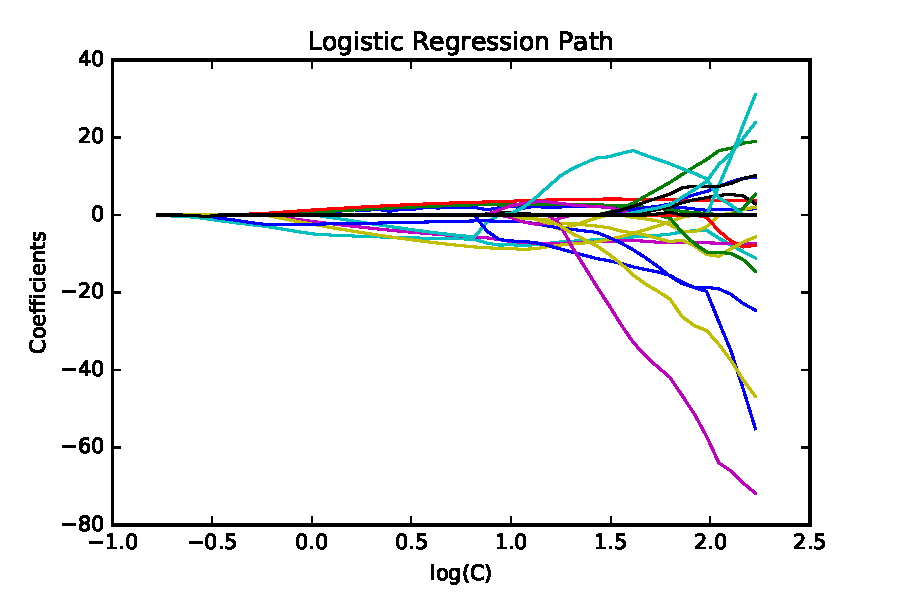
\includegraphics[scale=0.5]{fig5reg100.pdf}
\end{figure}


\subsubsection{with reg=1}
L2sklearn\\
Theta found by sklearn with L2 reg:  [ 1.1421394   0.60141117  1.16712554 -1.87160974 -0.91574144 -1.26966693
  0.12658629 -0.3686536  -0.34511687 -0.17368655 -1.42387465 -0.04870064
 -0.60646669 -0.26935562 -1.16303832 -0.24327026 -0.20702143 -0.04326335
 -0.28028058 -0.286921   -0.46908732 -1.03633961  0.02914775 -0.29263743
  0.01728096 -0.32898422 -0.13801971 -0.93196832]\\
Loss with sklearn theta:  0.46843403006\\

L1sklearn\\
Theta found by sklearn with L1 reg:  [ 1.86965269  0.68661649  1.28041683 -4.86256834 -1.6218069  -2.34227548
  0.          0.          0.          0.          0.          0.          0.
  0.         -2.36743001  0.          0.          0.          0.          0.
  0.          0.          0.          0.          0.          0.          0.
  0.        ]\\
Loss with sklearn theta:  0.438146984954\\
\begin{figure}[H]
  \caption{path}
  \centering
    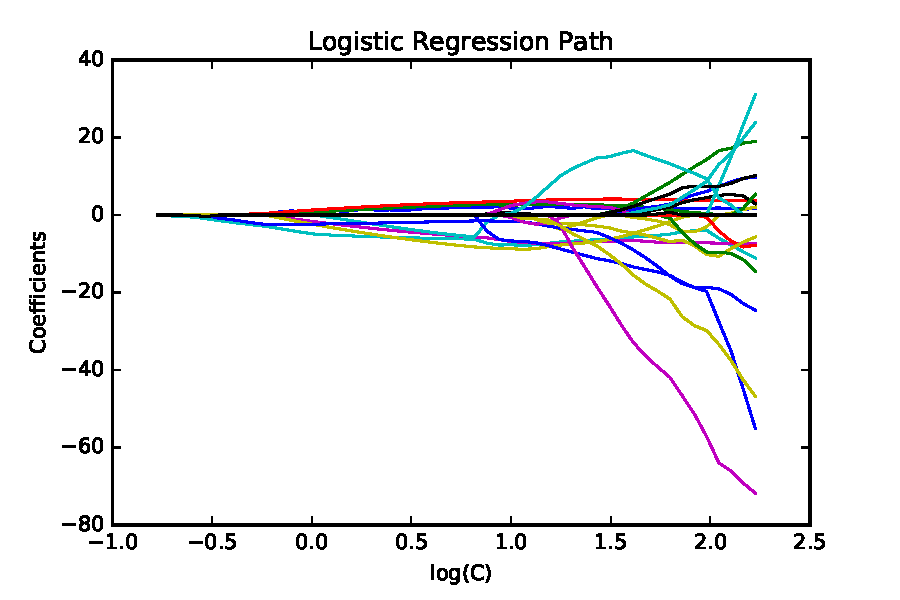
\includegraphics[scale=0.5]{fig5reg1.pdf}
\end{figure}


\subsubsection{with reg=0.1}
L2sklearn\\
Theta found by sklearn with L2 reg:  [ 2.65855183  1.76427994  2.91364412 -4.03385629 -3.34849756 -4.0181188
  0.76777199 -1.08648166 -0.47195071 -0.4774888  -3.27598952  0.54686285
 -1.80180787 -1.17932445 -2.79104067 -0.62127841 -0.4711418   0.61454641
 -1.14697992 -1.20796935 -0.10569617 -2.66246949  0.45857402 -0.76144039
  0.43744164 -1.17502213 -0.93753591 -1.20049576]
Loss with sklearn theta:  0.353830932899\\
L1\\
Theta found by sklearn with L1 reg:  [ 4.00273583  2.56793635  3.56332248 -7.68544357 -6.81244292 -8.6654482
  0.59001851 -0.20079995  0.          0.          0.          2.44529584
  0.          0.         -1.70280933  0.          0.          0.36834145
 -0.66643549  0.          0.         -6.7197063   0.          0.          0.
  0.         -0.05987662  0.        ]\\
Loss with sklearn theta:  0.336434280508\\
\begin{figure}[H]
  \caption{path}
  \centering
    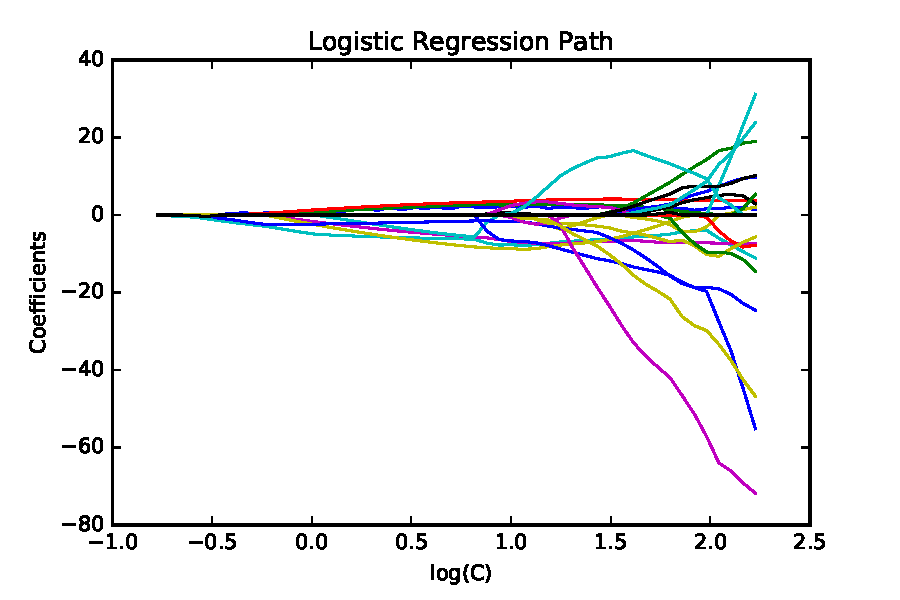
\includegraphics[scale=0.5]{fig5reg01.pdf}
\end{figure}


comment:
L1: When reg is increasing, the loss is increasing. The number of non-zero coefficients are decreasing, that means large reg makes more zero coefficients.
L2:When reg is increasing, the loss is increasing. Usually L2 won't give zero coefficients and we can see the value of theta is decreasing with larger reg.











\section{3PART C Logistic regression for spam classification}

L2 Penalty experiments -----------\\
best\_lambda =  0.1\\
Accuracy on set aside test set for  std  =  0.9296875\\

best\_lambda =  0.6\\
Accuracy on set aside test set for  logt  =  0.943359375\\

best\_lambda =  1.1\\
Accuracy on set aside test set for  bin  =  0.927734375\\


L1 Penalty experiments -----------\\
best\_lambda =  4.6\\
Accuracy on set aside test set for  std  =  0.921875\\

best\_lambda =  1.6\\
Accuracy on set aside test set for  logt  =  0.944010416667\\

best\_lambda =  3.6\\
Accuracy on set aside test set for  bin  =  0.92578125\\


Both L1 and L2 have best performance on logt with accuracy around 0.94.
For L2, when best lambda is increasing, the theat is decreasing.
L2 always give non-zero coefficients, while L1 give some zero coefficients.This is because L1 regularization forces coefficients to go to zero more often. 
L1 has larger sparsity than L2.
And we suggest to use L1 regularization because this model gives few parameters which is simper. We can get rid of irrelevant features and reduce the chance of overfitting.








\end{document}